\documentclass[11pt]{article}

% ACL style: "preprint" = non-anonymous with page numbers. Use "review" for an anonymous version, "final" for camera-ready.
\usepackage[preprint]{acl}

\usepackage{times}
\usepackage{latexsym}
\usepackage[T1]{fontenc}
\usepackage[utf8]{inputenc}
\usepackage{microtype}
\usepackage{inconsolata}
\usepackage{graphicx}
\usepackage{booktabs}
\usepackage{xcolor}
\usepackage{placeins}
\usepackage{adjustbox}
\usepackage{pdflscape}
\usepackage{pgfplots}
\pgfplotsset{compat=1.16}
\definecolor{cA}{HTML}{1F77B4}\definecolor{cB}{HTML}{E67E22}\definecolor{cC}{HTML}{2A9D8F}\definecolor{cD}{HTML}{8E44AD}\definecolor{cE}{HTML}{C0392B}
\pgfplotsset{vsplot/.style={vsbase, ybar, ymin=0}, vsbase/.style={bar width=9pt, width=\linewidth, height=4.6cm, axis lines*=left, axis line style={gray!70},
  ymajorgrids, major grid style={gray!25, line width=0.3pt}, tick style={gray!70}, tick label style={font=\footnotesize}, label style={font=\footnotesize},
  title style={font=\small\bfseries}, legend style={font=\scriptsize, draw=none, fill=none, at={(0.03,0.98)}, anchor=north west, legend columns=1, legend cell align=left}, enlarge x limits=0.35, nodes near coords, every node near coord/.append style={font=\scriptsize}}}
\hypersetup{hidelinks}
\renewcommand{\topfraction}{0.9}\renewcommand{\bottomfraction}{0.8}\renewcommand{\textfraction}{0.1}\renewcommand{\floatpagefraction}{0.75}\renewcommand{\dbltopfraction}{0.9}\renewcommand{\dblfloatpagefraction}{0.75}
\usepackage{tikz}
\usetikzlibrary{shapes.geometric,positioning,fit,backgrounds,arrows.meta,calc}

% ---------------------------------------------------------------- draft mode
% \todo{...} marks a number or fact still to be filled. Visible in the PDF while \drafttrue.
% For a clean copy set \draftfalse (the todo text then disappears; check that no sentence is left empty).
\newif\ifdraft
\drafttrue
\newcommand{\todo}[1]{\ifdraft{\textbf{[TODO: #1]}}\fi}

% ---------------------------------------------------------------- generated result tables
% Tables written by `python -m vakeel_sahayak.eval.scoring report` land in docs/results/dev-sweep/tables/.
% A missing file leaves a visible placeholder, so the document compiles with or without them.
\newcommand{\tabdir}{../results/dev-sweep/tables}
\newcommand{\resulttable}[2]{% #1 = file stem, #2 = "n" narrow (one column) or "w" wide (two columns)
  \IfFileExists{\tabdir/#1.tex}{%
    \begingroup
    \if#2w\let\table\table*\let\endtable\endtable*\let\small\scriptsize\fi
    \input{\tabdir/#1.tex}%
    \endgroup
  }{%
    \par\smallskip\noindent\fbox{\parbox{0.9\linewidth}{\footnotesize Table \texttt{\detokenize{#1}} not generated yet (scoring pipeline output).}}\par\smallskip
  }%
}

\newcommand{\gentable}[1]{\IfFileExists{generated/#1.tex}{\input{generated/#1.tex}}{\par\smallskip\noindent\fbox{\parbox{0.9\linewidth}{\footnotesize Table \texttt{\detokenize{#1}} not generated yet (run docs/report/tools/make\_result\_tables.py).}}\par\smallskip}}
\newcommand{\resref}[1]{\IfFileExists{\tabdir/#1.tex}{Table~\ref{tab:#1}}{the table \texttt{\detokenize{#1}}}}

\title{Vakeel-Sahayak.ai: An Agentic Harness for Bail Preparation\\ over Typed Legal Stores (Mid-Project Report, Version 1)}

\author{Vishak Kashyap K, Shravani K, Satvik Rao, Harshita Kumari \\
  International Institute of Information Technology, Hyderabad \\
  \texttt{vishakkashyap.k@research.iiit.ac.in}, \texttt{shravani.k@research.iiit.ac.in}, \\
  \texttt{satvik.rao@research.iiit.ac.in}, \texttt{harshita.kumari@students.iiit.ac.in} \\
  Code: \url{https://github.com/vishakkashyapk30/lma-group-project} (branch \texttt{midsub-report})}

\begin{document}
\maketitle

\begin{abstract}
Legal-aid lawyers in India prepare bail applications from messy case files: scanned and photographed orders, Hindi and English, several documents merged in one PDF. We describe Vakeel-Sahayak.ai, a bail-preparation engine built as an agent harness rather than a single model call. Six agents (intake, dossier and rights checks, retrieval orchestration, drafting, prosecution sparring, batch triage) work over ten typed stores on four shelves. An orchestrator reads a short evidence contract for each of twelve bail factors and decides which stores to query, in which order, and when to stop. Every claim in a draft is checked against its sources, and a draft changes only where a dependency changed. Two approval gates are enforced in code, and client text passes a pseudonymisation boundary before any external model sees it. We evaluate without manual annotation: gold labels come from court text, with a rule labeler and a non-Qwen model labeler that must agree and quote a verbatim span. We compare the full system with seven simpler baselines (single pass, single store, whole-document embeddings, naive chunking, query-every-store, a learned store router, and an expert rule list) and with 18 single-switch variants taken from recent agent and RAG papers. This report describes the system and the evaluation design, and states what has run so far. On the 50-case development set (OpenAI \texttt{gpt-6-luna}, hosted, earlier code) the full system's factor recall is 0.25 on the 8 orders that have a scorable gold factor, below the baselines (0.50 to 0.88) with no gap resolved; it is clearly ahead of the single-pass and single-store baselines on objection recall (0.69 against 0.00, 20 orders) and behind the query-every-store baseline (0.93), with an unsupported-fact rate of 0.87 against 0.76 to 0.98 for the baselines and a cost of about \$0.011 per case. These numbers are preliminary: small $n$, and development data only.
\end{abstract}

\section{Introduction}

\paragraph{Problem.} A legal-aid lawyer who prepares a regular bail application in an Indian High Court (CrPC s.439, now BNSS s.483) starts from a pile of documents: a born-digital High Court order, a scanned Sessions Court order, a phone photo of an FIR copy, remand orders and a custody certificate, often merged into one PDF and often in Hindi. The application needs exact statute text, a mapping from old to new sections since the 2024 change from IPC and CrPC to BNS and BNSS, court reasoning on each bail factor, the citation history of every authority, and the case's own timeline. No single vector index serves all of these. A model asked to write it from memory fabricates facts and case law, as studies of commercial legal research tools found \citep{magesh2025}.

The problem is one of data engineering and decisions before it is one of text generation: the input is heterogeneous, the knowledge has several shapes, each factor needs evidence from different places, the case keeps moving, and an office has hundreds of files to triage.

\paragraph{Why agentic.} Three of these steps involve a decision that depends on what was just found: how far down a parse ladder a page must go, which store to ask next for a given factor and whether the result is enough, and which part of a draft a new order has made stale. A fixed pipeline either does too much (every store, the vision model on every page) or too little. We built the decisions as agents with typed tools, typed hand-offs and budgets, and we measure each of them against a simpler alternative.

\paragraph{Scope.} Users are panel lawyers, junior advocates and supervised legal-aid clinics. The system does not predict outcomes, show grant rates, or advise accused persons or the public.

\paragraph{Contributions.} The research contribution is the harness and its evaluation, not a new model.
\begin{enumerate}\setlength\itemsep{0pt}
\item \textbf{The harness.} Six court-office agents over ten typed stores on four shelves; page-level agentic ingestion for ten input kinds; an orchestrator that plans retrieval per factor (Section~\ref{sec:system}).
\item \textbf{Evidence contracts.} For each of twelve bail factors, a short declarative list of the evidence a ground needs and which stores may hold it. The contract fixes what is needed and where it may be; the orchestrator decides the order, the query, sufficiency and the stop.
\item \textbf{Truth maintenance for drafts.} Each claim stores its dependencies. When counsel approves a change, only stale claims are redrafted and all other claims stay byte-identical, an idea from classical truth-maintenance systems \citep{doyle1979tms}.
\item \textbf{Two gates in code.} Counsel approves the dossier (Gate~1) and the brief (Gate~2). Export is impossible before Gate~2, and approvals can only come from counsel.
\item \textbf{Evaluation without manual annotation.} Seven kinds of gold label and nine test sets built from court text, official tables and construction; a sealed blind slice and a pre-registration; baselines B0 to B6; 18 single-switch variants from the recent agent and RAG literature, each with a switch, a paper and a test (Section~\ref{sec:eval}).
\end{enumerate}

\paragraph{Where the project stands, and how this report is organised.} This is a mid-project status report on work in progress, and there is a lot in it that already works. The system, the test sets, the scoring pipeline, a literature sweep of 18 single-switch variants and the pre-registered evaluation are built and tested. The 50-case baseline run and the Gemini-family runs are scored, and the retrieval, chunking and scheduling studies are measured. The results are small and are presented as a first look; the larger runs, the remaining variants and the blind slice belong to the next phase, which ends on 10 November. The report follows the order of the work. Section~\ref{sec:related} (related work) and Section~\ref{sec:literature} (the literature sweep) explain what we read, what ideas we took and why. Section~\ref{sec:system} describes the system and where each model runs, and Section~\ref{sec:data} the datasets. Section~\ref{sec:eval} sets out the baselines, ablations, metrics and statistics. Section~\ref{sec:results} gives the results so far, Sections~\ref{sec:challenges} to~\ref{sec:threats} the challenges, mitigations, limitations and threats to validity, and Section~\ref{sec:status} the progress, the work left and the timeline. The appendix holds the glossary, the arms, the metrics and the generated tables. The code is at \url{https://github.com/vishakkashyapk30/lma-group-project} (branch \texttt{midsub-report}, tag \texttt{dev-sweep-v3}).

\section{Related Work}
\label{sec:related}

\paragraph{Agentic and adaptive RAG.} Self-RAG and CRAG let the model critique retrieved text and re-retrieve \citep{asai2024selfrag,yan2024crag}; Adaptive-RAG chooses the retrieval depth by query complexity \citep{jeong2024adaptive}; Sufficient Context studies when the retrieved context is enough to answer \citep{joren2025sufficient}; HippoRAG~2 retrieves over a graph \citep{gutierrez2025hipporag2}. We implement adaptations of these as opt-in switches (S1, S2, S3, S5) and compare them with hand-written contracts. A related line routes among language models or answering agents \citep{zhang2026agentrouter}; our action space is about ten stores that are not agents, so a learned store prior is only one baseline (B5) and one ablation (S6).

\paragraph{Multi-agent systems and verification.} Self-critique without an outside verifier is reported to help little \citep{gou2024critic,huang2024selfcorrect}; we keep an NLI and rule-based check as the critic and add a self-critique arm (S8) to test this in our domain. For adversarial review, debate gains are partly explained by voting \citep{choi2025debate}, and context sharing can hurt \citep{wynn2025talk}. These motivate our prosecution-sparring ablations (S9, S10). \citet{cemri2025mast} give a taxonomy of multi-agent failures. AgentCourt and CourtEval place agents in court roles \citep{chen2025agentcourt,kumar2025courtevel}; our opponent is scored against objections the real prosecution raised.

\paragraph{Ingestion and chunking.} VisRAG and ColPali retrieve over page images \citep{yu2025visrag,faysse2025colpali}; we use an image-only arm as a baseline for a text-first routing ladder. Dense X Retrieval studies the granularity of retrieval units \citep{chen2024densex}; our naive-chunking baseline B3 and the proposition-unit variant S16 test this on court orders.

\paragraph{Legal NLP.} Work on Indian courts is mostly judgment or outcome prediction \citep{nigam2025nyayarag,nigam2024predex}. \citet{magesh2025} show that commercial legal RAG tools still fabricate and misground citations. We cite them for positioning and design the metrics around that finding: every citation is looked up, and every quoted span must appear verbatim in the cited paragraph. Counter-argument retrieval as a separate kind of evidence \citep{wachsmuth2018} motivates our authority-stance variant (S18).

\paragraph{Evaluation.} For grounding we use MiniCheck \citep{tang2024minicheck} and an NLI model, and citation precision and recall in the style of ALCE \citep{gao2023alce}. No score in this report comes from an LLM judge.

\paragraph{Safety and serving.} Typed hand-offs follow design patterns for securing agents \citep{beurerkellner2025patterns}; batch scheduling follows serving work such as SGLang \citep{zheng2024sglang}. Both are opt-in arms (S17, S14).

\section{Literature Sweep and Its Tests}
\label{sec:literature}

The design of the system was not fixed once. Four sweeps through the literature (retrieval and orchestration; verification and adversarial review; intake, safety and serving; routing, topology, chunking and workflow search) each produced a list of ideas that a paper reported as useful, and each idea became an opt-in \emph{variant} of the harness. This section records which paper each variant comes from, what was changed when the idea moved to a bail-preparation setting, and what has been checked about it so far. The full table, with links, is \texttt{docs/literature-to-code-map.md} in the repository.

\paragraph{Rules of the sweep.} (1) Every variant is a field of one typed \texttt{Switches} object and defaults to the current behaviour; a golden test per agent (digests of the default run of case-0007, captured before any variant was written) fails if switching a variant off does not reproduce the old output byte for byte. (2) A variant is an \emph{adaptation}, never a reproduction: each row of the map says what was replaced (for example, the learned complexity classifier of Adaptive-RAG became deterministic rules over the Rights Radar and the statute era). (3) A variant is built only if it can be scored by a metric of the evaluation plan; its row names the claim, metric and test file. (4) Constants that the papers do not give (the skew thresholds of S4, the damping and depth of the graph expansion of S5) are marked as untuned assumptions to be set on the dev split, never on the test split. (5) No variant is claimed to help until it has been scored against Full on the same backend and cases (Section~\ref{sec:results}).

\paragraph{Citation check.} Every paper in the map was checked against the official proceedings page or the arXiv record. Four links or author lists were corrected (Self-RAG, CRITIC, the first author of the multi-agent failure taxonomy, and a preview link for semantic chunking); seven further checks passed, one with a note on a changed page title; Doyle's truth-maintenance paper was checked on secondary sources only, and its row says so. Preprints without a venue are labelled as such.

\subsection{How the literature review was done}
\label{sec:litprocess}

\paragraph{Why we reviewed the literature.} Our project is an engineering contribution: the way agents, stores, checks and approval gates are put together for one workflow. Such a claim is only credible if each design choice is placed against published work (what is borrowed, what is adapted, what is new) and if each borrowed idea becomes a test that can fail. The review therefore had two outputs, a catalogue of papers with a recorded decision for each, and a map from papers to code switches and metrics (Table~\ref{tab:literature}). It also had a third, less visible output: a list of ideas we looked at and did not adopt, with the reason.

\paragraph{Scope and search.} We covered fourteen themes: routing among models; multi-agent orchestration and its failure modes; agentic and adaptive retrieval-augmented generation; graph-structured and multi-source retrieval; document ingestion and chunking; verification, attribution and self-correction; debate and adversarial critics; memory and state; agent safety; agent evaluation; legal AI and Indian legal NLP; clarification, abstention and human-in-the-loop; small models and structured output; serving and scheduling. We searched 2023 to 2026 proceedings (ICML, ICLR, NeurIPS, ACL, EMNLP, NAACL, COLM, AAAI, IJCAI, SIGIR, ICAIL, USENIX, OSDI, MLSys, TMLR, TACL) and arXiv for items without a venue, starting from the two papers the course team named and from the TA's request for novelty in agentic engineering rather than in a new model.

\paragraph{Three passes, and how each paper was checked.} A first sweep per theme recorded candidates with an official link. A second pass checked 33 papers one by one against the official page (proceedings, ACL Anthology or arXiv). A third pass re-fetched 25 more, including the two named papers, and corrected several venue claims; where a venue could not be confirmed (for some preprints and workshop papers) the entry says so instead of guessing. Each catalogue row carries a check mark (verified on an official page, or taken from the sweep only), a tier (top venue, workshop or other, preprint) and a relevance score from 1 to 5 that records how much the paper changes a decision in this project.

\paragraph{What the catalogue holds.} 145 papers: 114 from a top venue, 8 workshop or other, 23 preprints; 34 score 4 or 5 and form the core reading list, 81 score 3 (a useful idea), and 30 score 1 or 2 (framing only). A further 24 were read and not catalogued. Contribution lines come from abstracts and earlier summaries, not from full reads of every paper, and the numbers papers report (for example attack success rates) are theirs, on their benchmarks; nothing in the review is evidence about our own system.

\begin{table*}[!t]
\centering\small
\begin{adjustbox}{max width=\textwidth}
\begin{tabular}{@{}p{3.1cm}p{4.9cm}p{6.6cm}@{}}
\toprule
Kind of paper & Examples & What we took, and why \\
\midrule
Adaptive retrieval and sufficiency & Self-RAG, CRAG, Adaptive-RAG, Sufficient Context \citep{asai2024selfrag,yan2024crag,jeong2024adaptive,joren2025sufficient} & Sutradhar stops when the evidence for a factor is enough, and caps effort by case complexity (S3, S6). Chosen because stopping and sufficiency are the closest match to the orchestrator's job; their trained components were replaced by rules over the Rights Radar and the statute era, since we have no routing labels. \\
Graph and multi-source retrieval & HippoRAG~2, ToG~2.0, HybGRAG, GraphRAG, LightRAG & A citation graph extracted from the orders themselves, expanded by personalised PageRank (S5); the entity-graph systems built by LLMs were left out for indexing cost, and a paper reporting that graph RAG often loses to plain RAG is the reason S2 is a small ablation. \\
Verification and self-correction & CRITIC, ``Cannot Self-Correct'', MiniCheck, ALCE \citep{gou2024critic,huang2024selfcorrect,tang2024minicheck,gao2023alce} & Self-critique without an outside verifier helps little, so Vakeel repairs with an NLI and rule check, and a self-critique arm (S8) tests that claim here. MiniCheck scores the unsupported-fact rate; ALCE-style citation precision and recall score citations. \\
Debate and critics & Debate or Vote, MAD, Talk Isn't Always Cheap \citep{choi2025debate} & Several studies find debate gains come from voting. So Abhiyojak (the prosecution critic) must beat a sampling-only critic at equal tokens (S9), and context isolation is an ablation (S10). \\
Ingestion and chunking & VisRAG, ColPali, Dense X \citep{yu2025visrag,faysse2025colpali,chen2024densex} & A text-first page ladder with an image-only baseline (P7); propositions as retrieval units (S16) against naive chunking (B3). \\
Agent safety & Design Patterns for Securing Agents, CaMeL \citep{beurerkellner2025patterns} & Prompt injection is an architecture problem. Typed hand-offs and code-enforced approval gates fit; the injection-defence variant S17 and the hidden-text check on PDFs follow from this. \\
Agent evaluation & AI Agents That Matter, $\tau$-bench & Cost and reliability beside accuracy: tokens, store calls and pass$^k$ are reported for every arm, never one accuracy number. \\
Legal AI for India & NyayaRAG, PredEx, ``Hallucination-Free?'' \citep{nigam2025nyayarag,nigam2024predex,magesh2025} & Indian work is mostly outcome prediction, which the system refuses by design. We position as preparation with checked citations, where commercial legal RAG tools were shown to fabricate, and make the citation checks the headline safety metrics. \\
Serving and scheduling & SGLang, KV-cache scheduling \citep{zheng2024sglang} & Plan caching and an urgency-ordered batch queue (S14), applied at the application level because we cannot modify a serving engine. \\
\bottomrule
\end{tabular}
\end{adjustbox}
\caption{Kinds of papers reviewed, the inspiration taken and the reason. The full catalogue is in the project repository (\texttt{docs/literature-review-and-usage.md}).}
\label{tab:litkinds}
\end{table*}

\paragraph{What we did not adopt, and why.} The reasons are specific to our constraints: open-weight or free-tier models at run time, small GPUs, no manual annotation, eight weeks, and the need for an auditable legal record. (a) Trained routers, searchers and stoppers (Router-R1, Search-R1, AutoSearch) need rollouts or routing labels we do not have; we kept their loop shape and their cost-aware reward as evaluation ideas and left the policy to rules and contracts. (b) Automated workflow search (AFlow, ADAS, MaAS) spends thousands of model calls and returns pipelines that are hard to audit; only difficulty-adaptive effort was borrowed. (c) Memory managed by a language model (MemGPT, Mem0) conflicts with an event-sourced case record that must be auditable. (d) Vision-first retrieval as the main path needs a vision model on every page and stays a baseline. (e) Training-based and detector-style injection defences were replaced by architecture. (f) Outcome-prediction systems conflict with the rule that the system gives no outcome predictions or grant rates. (g) Other-jurisdiction legal benchmarks use US or Chinese law, so only their metric ideas were kept.

\paragraph{Findings that changed the design.} Five findings changed what we built. Stopping and sufficiency checks are the most direct match to the orchestrator, so rule checks plus a rater are tested while a trained stopper is not built. Self-correction needs outside evidence, so the repair loop uses an NLI and rule check, with a self-critique comparison. Debate is not better than sampling at equal cost, so the prosecution critic carries the burden of proof. Prompt injection is an architecture problem, which favours typed hand-offs. Agent evaluation needs cost and reliability, so every table carries tokens, store calls and pass$^k$.

\paragraph{Limits of the review.} Every idea we borrowed was written for other tasks and mostly other models, so each is an adaptation and a hypothesis here, not a result. Many 2026 items are preprints. The review is the reason each switch exists; whether a switch helps is decided only by the runs in Section~\ref{sec:results}, and null or negative results will be reported as such.

\subsection{What was built, by sweep}

\begin{table*}[!t]
\centering\footnotesize
\begin{adjustbox}{max width=\textwidth}
\begin{tabular}{@{}p{2.2cm}p{3.5cm}p{3.6cm}p{4.6cm}r@{}}
\toprule
Variant & Idea (paper) & Switch & What was adapted & Tests \\
\midrule
\multicolumn{5}{@{}l}{\textit{Sweep 1: retrieval and orchestration (Sutradhar, stores)}} \\
S3, S3b & Stop when the evidence is sufficient (Sufficient Context; AutoSearch; Stop-RAG) & \texttt{stopping} = rules, rules\_llm, llm & Rules first, a model rating second; stopped-too-early and over-search are scored (M18) & 20 \\
S1 & Critique retrieved text, re-retrieve on a miss (Self-RAG; CRAG) & \texttt{retrieval\_policy} = self\_critique & A slot with nothing retrieved is MISSING and costs no critic call; verdicts kept in the event log & 24 \\
S2 & Retrieval depth by complexity (Adaptive-RAG) & \texttt{retrieval\_policy} = adaptive & Classifier replaced by rules: none, single, multi; round cap per factor & 21 \\
S5 & Expand over a citation graph (HippoRAG 2) & \texttt{graph\_expansion} & Personalised PageRank on 5,842 citation edges; expanded paragraphs must still pass the slot rules (factor, family, date) & 33 \\
S4 & Score skew as weak-evidence signal (SkewRoute) & \texttt{weak\_signal} = skew & Gini and top gap of the fused scores; thresholds untuned & 23 \\
\multicolumn{5}{@{}l}{\textit{Sweep 2: verification and adversarial review (Vakeel, Abhiyojak)}} \\
S8 & Self-critique without an outside verifier (CRITIC; ``cannot self-correct yet'') & \texttt{repair\_mode} = self\_critique & Replaces the NLI and rule check by the drafter's own critique, to test the claim in this domain & 16 \\
S9 & Sampling-only critic at equal tokens (Debate or Vote; ``Should we be going MAD?'') & \texttt{critic\_mode} = sampling & Same token budget as the critic, spent on samples & 21 \\
S10 & Debate without context isolation (``Talk Isn't Always Cheap'') & \texttt{abhiyojak\_isolation} = off & Abhiyojak sees Vakeel's reasoning; flip rate measured & 11 \\
S11, S11b, S11c & Grader, critic, defender (CourtEval); two-instance debate; three-sample vote & \texttt{critic\_mode}, \texttt{draft\_mode} & Roles mapped to the sparring and drafting steps & 18 \\
S15, S15b & Reasoning before structured output; free text then parse (``Let Me Speak Freely?''; CRANE) & \texttt{output\_format} & Schema-valid rate, repairs and tokens compared across the three layouts & 17 \\
S18 & Authority stance: counter-argument evidence (Wachsmuth et al.) & \texttt{authority\_stance} = outcome & Supporting authorities first, precedents from refused orders flagged & 6 \\
\multicolumn{5}{@{}l}{\textit{Sweep 3: intake, safety and serving (Munshi, defences, Pairokar)}} \\
S17 & Prompt-injection defences: typed hand-off, spotlighting, guard (design patterns for securing agents) & \texttt{no\_typed\_handoff} and two more & Each defence can be switched off; attack success scored on T7 & 10 \\
S7, P7, P8 & Hierarchy-ranked gap re-reading (IntrAgent); image-only ingestion (VisRAG, ColPali); keep weak text layer & \texttt{munshi\_gap\_policy}, \texttt{munshi\_image\_only}, \texttt{munshi\_keep\_weak\_text} & Pages re-read per recovered field; vision calls per page & 41 \\
S14, S14b--d & Plan caching, scheduling, prefix-friendly prompts (Agentic Plan Caching; SGLang) & \texttt{plan\_cache}, \texttt{urgency\_policy}, \texttt{prefix\_layout} & Second case with the same signature skips all 8 planning calls: 30,633 to 12,836 tokens, packs byte-identical & 38 \\
\multicolumn{5}{@{}l}{\textit{Sweep 4: routing, topology, chunking, workflow search}} \\
S6, B5 & Learned store prior (GraphRouter; AgentRouter) & \texttt{store\_prior} = order, only & Orders calls inside a contract, or replaces it; artefact not yet trained on real data & 17 \\
S12, S12b & Orchestrator-worker topology (scaling agent systems; MAST) & \texttt{topology} & Lock-step vs sequential vs one merged agent & 11 \\
S16, S16b & Chunk granularity, propositions, late chunking (Dense X) & \texttt{chunking} & Fixed, recursive, semantic, page, proposition & 22 \\
S13 & Automatically designed workflows (AFlow; ADAS) & grid over switches & Budget-capped grid search on dev; harness and offline smoke only & 14 \\
\bottomrule
\end{tabular}
\end{adjustbox}
\caption{Ideas taken from the literature, the switch that turns each on, how it was adapted, and the number of unit tests that pin it. Test counts are those of the files named in \texttt{docs/literature-to-code-map.md}; they are collected, not re-run, in this table.}
\label{tab:literature}
\end{table*}

\subsection{How the variants are tested}

The tests answer four different questions, and a variant is not called done until all four have an answer.

\paragraph{1. Does the default stay the same?} Each of Sutradhar, Vakeel, Peshkar and Munshi has a golden test that hashes the evidence packs, plans, event multiset, budget, prompts and drafted output of the default run (Peshkar over a planted shelf, Munshi over the 14-page bundle). Adding a variant must not change a digest. This is the test that lets 46 switches coexist with the shipped behaviour.

\paragraph{2. Does the switch do what the paper's idea says?} Each variant has its own test file, 631 collected unit tests across 37 files (about 220 of them are the shared registry, switch and effect tests) (Table~\ref{tab:literature}). They check mechanism, not quality: the critique variant issues no critic call for an empty slot; the adaptive policy caps rounds for single-factor cases (case-0007 is a BNS-era case, so every factor is ``multi'' there and the single and none branches are tested by reading it as IPC-era); graph expansion only counts a hit that also passes the factor, family and date rules; the Gini and top-gap signals are computed on scored searches that leave the unscored path unchanged. A registry test fails if a variant id appears in the plan without a switch, a map row, or a test, and an end-to-end audit runs every one of the 61 ids through the offline pipeline (61 of 61 pass; 42 have a measured-effect test that checks the switch changes the run in the direction the idea predicts).

\paragraph{3. Is it measured on the right metric?} Each row names a metric from the evaluation plan: stopped-too-early and over-search (S3), verdict counts (S1), tokens and store calls at equal recall (S2, S14), recall@10 of the citation graph with and without expansion (S5), AUROC of the score skew against ``the top ten contain a cited precedent'' (S4), unsupported-fact rate and repair success (S8, S15), objection recall at equal tokens (S9, S10, S11), pages re-read per recovered field (S7), attack success (S17). A scoring test pins the metric on synthetic inputs with known answers, so a metric change cannot pass silently.

\paragraph{4. Is the claim tied to the right comparison?} A variant is compared only with Full on the same backend and cases; the scorer refuses mixed code stamps and scores one model family per backend, applies a Holm correction inside each family of claims, and decides the headline claim by an intersection-union rule (every comparator must lose). A comparator that was not run makes the claim ``incomplete'', not ``supported''.

\subsection{What has been measured so far}

Mechanism tests and the 61-id audit are complete and green (5,082 passed on 29 October). Quality measurements are fewer, and we state them as they stand.

\paragraph{S4 and S5 on the real stores (offline, no model).} On a self-supervised proxy of 150 queries (a held-out citing order, with its cited precedents as targets under a strict before-date filter), expanding the citation graph raised recall@10 from 0.037 to 0.537; the paired difference is 0.50 (95\% interval 0.42 to 0.58, McNemar $p<10^{-20}$; 75 queries gained and none lost). The gain comes from co-citation structure rather than from the retriever finding the cited order itself, and the proxy is optimistic, so this is evidence that the graph carries signal, not a forecast of the gain on real briefs. The score-skew signal separates queries with and without a cited precedent in the top ten with an AUROC of 0.870 (interval 0.751 to 0.969); as a weak-evidence flag at the chosen threshold it has precision 1.0 and recall 0.49. The second query set (G2, the precedents the court cited) has only 8 queries and no positives, so no claim is made on it.

\paragraph{Caching, scheduling and chunking.} Plan caching on case-0007 (offline): the second case with the same signature skips all 8 planning calls, tokens fall from 30,633 to 12,836 and the evidence packs are byte-identical to the no-cache run. The scheduling and chunking studies run as simulations or on self-supervised targets and say so in their output; they are reported as such, not as serving measurements.

\paragraph{Measured on a model, and not yet.} The retrieval, chunking and scheduling variants (S4, S5, S14, S16) are measured without a model; Section~\ref{sec:results} reports them. Ablation A1 and the baseline B0L have run in the Gemini family and are scored there. Most of the other variants and ablations (S1 to S6, S8 to S12, S15, S18, A1 to A3, A6 to A9) have run against Full on an OpenAI backend at 10 to 30 dev cases; their scores are not in this version, and at those sizes most differences would be inside the intervals, so we will read them as a first look and not as a ranking. Not yet run on a model: S7, S11b and c, S12b, S13, S15b, S17, P5 to P8 and A4, A5 and A10; they are in the timeline to 10 November (Section~\ref{sec:status}). A null or negative result on any variant will be reported as such.

\section{System}
\label{sec:system}

Figure~\ref{fig:arch} shows the system. The agents are named after people in an Indian court office, and each has a narrow decision to make.

\begin{figure*}[!t]
\centering
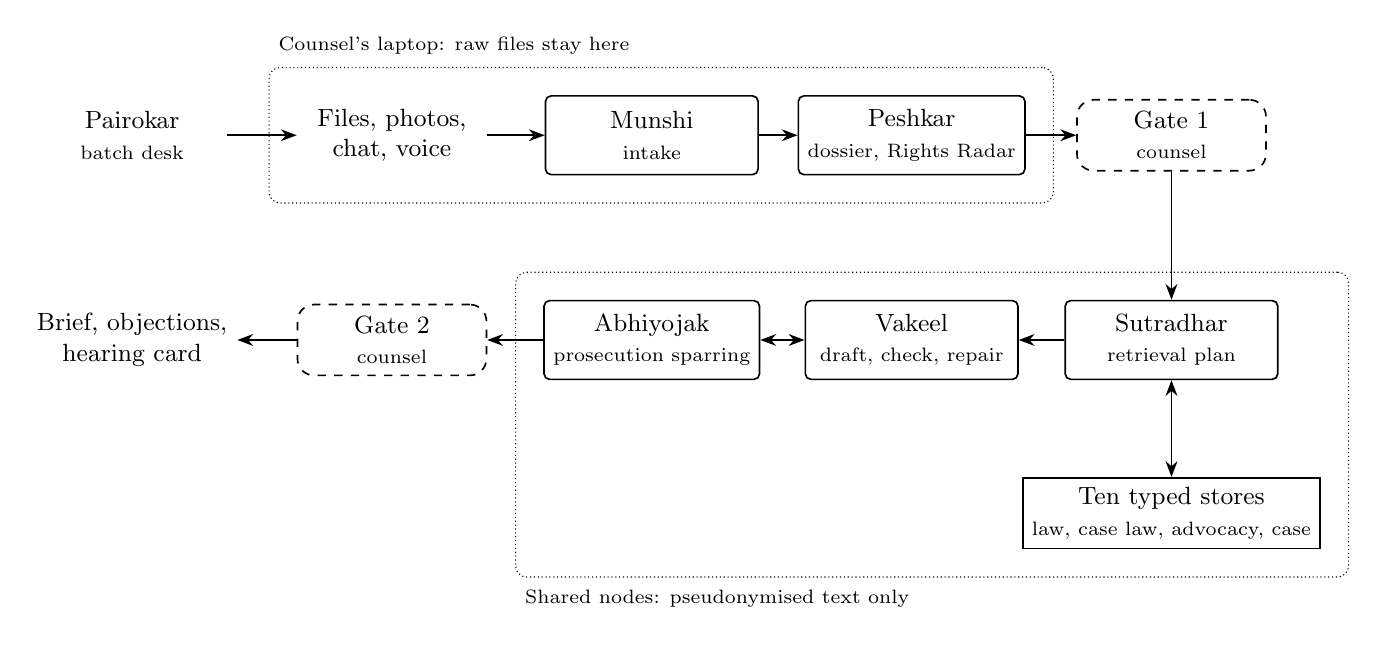
\begin{tikzpicture}[
  font=\small, >=Stealth, line width=0.6pt,
  ag/.style={draw, rounded corners=2pt, align=center, minimum width=2.7cm, minimum height=1.0cm},
  st/.style={draw, align=center, minimum width=3.4cm, minimum height=0.9cm},
  gt/.style={draw, dashed, rounded corners=6pt, align=center, minimum width=2.4cm, minimum height=0.9cm},
  io/.style={align=center, minimum width=2.4cm}]
% row 1: counsel's laptop, left to right
\node[io] (pa) at (0,0) {Pairokar\\{\scriptsize batch desk}};
\node[io] (in) at (3.3,0) {Files, photos,\\chat, voice};
\node[ag] (mu) at (6.6,0) {Munshi\\{\scriptsize intake}};
\node[ag] (pe) at (9.9,0) {Peshkar\\{\scriptsize dossier, Rights Radar}};
\node[gt] (g1) at (13.2,0) {Gate 1\\{\scriptsize counsel}};
% row 2: shared nodes, right to left
\node[ag] (su) at (13.2,-2.6) {Sutradhar\\{\scriptsize retrieval plan}};
\node[ag] (va) at (9.9,-2.6) {Vakeel\\{\scriptsize draft, check, repair}};
\node[ag] (ab) at (6.6,-2.6) {Abhiyojak\\{\scriptsize prosecution sparring}};
\node[gt] (g2) at (3.3,-2.6) {Gate 2\\{\scriptsize counsel}};
\node[io] (out) at (0,-2.6) {Brief, objections,\\hearing card};
% row 3: stores
\node[st] (stores) at (13.2,-4.8) {Ten typed stores\\{\scriptsize law, case law, advocacy, case}};
\draw[->] (pa) -- (in); \draw[->] (in) -- (mu); \draw[->] (mu) -- (pe); \draw[->] (pe) -- (g1);
\draw[->] (g1) -- (su);
\draw[->] (su) -- (va); \draw[<->] (va) -- (ab); \draw[->] (ab) -- (g2); \draw[->] (g2) -- (out);
\draw[<->] (su) -- (stores);
\begin{scope}[on background layer]
 \node[draw, densely dotted, rounded corners, fit=(in)(mu)(pe), inner sep=0.35cm] (lap) {};
 \node[draw, densely dotted, rounded corners, fit=(su)(va)(ab)(stores), inner sep=0.35cm] (srv) {};
\end{scope}
\node[font=\scriptsize, anchor=south west] at ([yshift=1pt]lap.north west) {Counsel's laptop: raw files stay here};
\node[font=\scriptsize, anchor=north west] at ([yshift=-1pt]srv.south west) {Shared nodes: pseudonymised text only};
\end{tikzpicture}
\caption{Architecture. Arrows show the order of work; the double-headed arrows are request and reply. Dotted boxes mark where each part runs; dashed boxes are the two approval gates, which only counsel can open and which are enforced in code, so nothing is exported before Gate 2.}
\label{fig:arch}
\end{figure*}

\paragraph{Agents.} \textbf{Munshi} (intake) decides the parse route of each page, when to escalate, document boundaries and types, where each item is filed, and what is missing. \textbf{Peshkar} builds the dossier with a source quote for every field, a List of Dates, and the Rights Radar (deterministic checks on custody periods and statutory rights, each with a verification status). \textbf{Sutradhar} orchestrates retrieval. \textbf{Vakeel} drafts the grounds and checks and repairs every claim. \textbf{Abhiyojak} plays the prosecution with its own prompt and an allow-listed context. \textbf{Pairokar} orders a batch by urgency and decides per case between a full brief, a flag for counsel, or a request for documents. Every action is appended to an event log; dossier, timeline, brief and sparring record are views of it, which gives an audit trail and the dependency data for truth maintenance.

\paragraph{Ingestion ladder.} Munshi handles ten input kinds (born-digital, scanned, degraded, phone photo, Hindi or mixed script, legacy Hindi fonts, handwriting, bundles, locked files, non-PDF). A page climbs only as far as needed: text layer; layout parser; clean-up and OCR; a vision model asked only to transcribe; a request to counsel for a clearer copy. Per-page quality signals (text coverage, OCR confidence, dictionary-word share, script, legacy-font patterns) decide each step and are logged. A gap-driven re-read returns to a page when a checklist field is still missing. The ladder is evaluated as a router against the cheapest route that clears the quality bar.

\paragraph{Ten stores on four shelves.} A brief needs exact text, a section-mapping graph, court reasoning, citation history, what each side usually argues, and the client's own record; each has a different right way to search. The \emph{law} shelf holds statutes (exact lookup, BM25) and the IPC--BNS and CrPC--BNSS concordance (typed graph). The \emph{case-law} shelf holds reasoning paragraphs (BM25 plus a dense vector, metadata pre-filter), the citation graph with treatment and court level, and whole-order fact vectors. The \emph{advocacy} shelf holds defence-argument and prosecution-objection paragraphs by factor, used for coverage and phrasing, never cited as authority. The private \emph{case} shelf holds the client's documents in structure-aware chunks, a dated timeline and the dossier. The October 2026 build has 161,708 reasoning paragraphs, 70,880 arguments, 55,161 objections, 114,692 similar-fact orders and 5,842 citation edges (37.3\% of citations resolved to a document). Test-window orders and same-FIR orders are excluded from every store. The dense side of the runs reported here is a hashed character n-gram vector, not BGE-M3; BGE-M3 side vectors for the four vector stores were built afterwards on a GPU node (2\,h\,43\,min, 1.65\,GB) and are opt-in (\texttt{VS\_STORES=bge}); retrieval under BGE-M3 is not yet measured.

\paragraph{Evidence contracts and the orchestrator.} Each of twelve bail factors has a contract: slots (for example co-accused order, role comparison, authority, good-law check, likely objection), a need for each (required, a count, or optional), the stores that may hold it, and a budget in store calls and tokens. Sutradhar decides whether the factor applies, the order of calls, the query and filters, whether a result is good enough, when to relax a filter or follow a citation, and when to stop; slots left unfilled become open issues, never silent omissions. A learned store prior, trained from train orders, may order calls within a contract (S6) or replace the contracts (B5).

\paragraph{Checking and truth maintenance.} Vakeel checks every claim with an NLI model and rules (statute lookup, section mapping, good-law check), and repairs or flags it; nothing is dropped silently. Each claim records the dossier fields (by hash), timeline events, rights entries and authorities it depends on. When counsel approves a change, claims with a changed dependency, and claims citing them, become stale; only the reopened factors are re-planned, and unchanged claims stay byte-identical (tested).

\paragraph{Gates and privacy.} Gate 1 (dossier) and Gate 2 (brief) pass only on counsel's approval, and export is impossible before Gate 2, in code and in tests. Raw client files stay on the user's machine. External model services are off by default, gated by a mode (\texttt{off}, \texttt{public}, \texttt{pseudonymised}, \texttt{consented}); client text needs counsel's per-case consent event for the provider even when pseudonymised, and every external payload passes the boundary. The boundary aliases names and quasi-identifiers (FIR, case and crime numbers, police stations, villages, addresses, PIN codes, vehicle numbers, ages) and shifts every date by a per-case offset; on the 250 T1 orders no FIR number, case number or numeric date survived, and the boundary refused 5 orders whose names were glued to other words by OCR (those calls stay local). Gate 2's approval is bound to a hash of the brief, sparring record and List of Dates, so a later change re-closes export. Defences against instructions planted in documents (a typed hand-off from a tool-less extractor, spotlighting, a guard) are all on by default; switching each off is an arm of the safety test set T7.

\paragraph{Models and where they run.} The design specifies a 4B model with OCR and a vision model on an 8\,GB laptop GPU for Munshi and Peshkar, and a 14B model on shared GPU nodes for Sutradhar, Vakeel and Abhiyojak. None of the runs reported here used those: serving a 32B model on the shared nodes failed (Section~\ref{sec:challenges}), so every language-model run is either hosted or an offline stand-in. Table~\ref{tab:models} lists each block of runs with its provider, model and where it executes. Hosted calls go only through the pseudonymisation boundary; the Gemini free tier receives public court text only. Paid providers are locked in code and were opened for OpenAI alone, for the block marked below, with the owner's go-ahead and a spend cap.

Table~\ref{tab:models} (Appendix~\ref{app:models}) lists, for every block of runs, the provider, the model and whether it ran locally or on a hosted service.

\section{Datasets}
\label{sec:data}

All data are public court text, official tables, existing datasets, or constructed; no client data and no hand-made labels are used (Table~\ref{tab:data}).

\paragraph{Corpus.} Open India Law (release v2026.08.1) supplies the court orders: bail-related High Court decisions from 2019 to 2025 and Supreme Court judgments of any year (1.4\,GB of the 53.6\,GB release). Of 115,988 orders read, 115,524 feed the stores; 464 are excluded because they are test-window orders or share an FIR with one. Orders dated before 2024 are the training window; the test window is later. IPC2BNS-Verify supplies the IPC-to-BNS concordance (563 rows) and a 1,140-query mapping benchmark. Statute texts come from the corpus's legislation file (IPC, BNS, BNSS) plus the CrPC and NDPS sections the rules need, 1,426 sections in all. Kathbath (first 1,000 of 3,130 Hindi test utterances) supplies Hindi speech for dictated facts.

\paragraph{Stores.} The build of 26 October 2026 took 35 minutes on a laptop and holds 1.77\,GB: 161,708 reasoning paragraphs, 114,692 whole-order fact vectors, 70,880 defence-argument and 55,161 prosecution-objection paragraphs, and 5,842 citation edges (37.3\% of extracted citations resolve to a document in the index).

\paragraph{Test sets.} T1 is the main set: 200 test-window High Court orders (120 open after the freeze, 80 blind) and 50 development orders; the system reads the facts part of each order and gold comes from the rest of it (Section~\ref{sec:eval}). The facts part is short: 19 of the 50 dev orders have under 1,000 characters of facts, and one has only the caption. T2 to T9 test the other parts of the system.

\begin{table}[!t]
\centering\small
\begin{adjustbox}{max width=\textwidth}
\begin{tabular}{@{}llr@{}}
\toprule
Set & Content & Size \\
\midrule
T1 & HC bail orders, facts in, gold out & 200 + 50 dev \\
T2 & messy bundles; native Hindi orders & 600; 200 \\
T3 & change-set updates & 240 \\
T4 & rights scenarios (rule table) & 627 \\
T5 & batch cases, planted deadlines & 300 \\
T6 & chat questions & 150 \\
T7 & safety scenarios & 60 \\
T8 & Hindi utterances & 300 \\
T9 & citation strings & 2,095 \\
\bottomrule
\end{tabular}
\end{adjustbox}
\caption{Test sets on 29 October 2026 (rows on disk). T2, T3, T5, T7 and T8 are constructed with known answers; T4 is generated from the written rule table.}
\label{tab:data}
\end{table}

\section{Evaluation Design}
\label{sec:eval}

The evaluation follows the course material on evaluation (L12) and on RAG evaluation (L14): state the evaluated object, decide the claims, thresholds and tests before looking at results, seal a slice, report intervals, and audit the metrics themselves. No score comes from an LLM judge, and no label is made by hand.

\paragraph{Test sets.} Nine sets built from court text, official tables or construction. \textbf{T1}: 200 High Court test-window orders (at least 60 BNS-era), facts part as input, plus 50 dev orders. \textbf{T2}: 600 messy bundles with known text, boundaries and fields, and 200 native Hindi High Court orders. \textbf{T3}: 240 change-set updates. \textbf{T4}: 627 rights scenarios from the written rule table (a conformance check of the Radar against its specification, not a legal one). \textbf{T5}: 300 batch cases with planted deadlines. \textbf{T6}: 150 chat questions. \textbf{T7}: 60 safety scenarios. \textbf{T8}: 300 utterances (Kathbath Hindi, dictated facts). \textbf{T9}: 2,095 citation strings.

\paragraph{Gold labels without annotators.} Seven kinds of gold label are derived from the order text. G1 is the set of the 12 bail factors the defence argued; G2 the precedents the court cited that resolve to a document in the index; G3 dossier fields and dated events (sections, dates, charge-sheet status, co-accused bail, stage); G4 the objections the prosecution raised; G5 the factors the court discussed; G6 condition types of the operative order; G7 the rights computations the court states itself (custody against the 60 and 90 day limits, s.436A and s.479). For G1 and G3 (and, with weaker coverage, G4 to G6) two labelers work independently: the keyword and date rules, and a hosted model (OpenAI \texttt{gpt-6-luna}) that is not shown the rule output. This labeler is the same model as the system in the dev runs, so the agreed gold is not independent of the system; the rule-only gold is therefore reported beside it as a co-primary column. A label enters gold only if both agree, and the labeler must quote a verbatim span, which is rejected unless it is found in the order (a date label needs a written date in the span that normalises to the claimed date). The agreed gold is primary; the rule-only gold is a declared secondary, and every headline metric is also recomputed on it (label-source sensitivity). Table~\ref{tab:kappa} gives agreement on 250 orders (200 test plus 50 dev); a second labeler (Sarvam-105B) on a random 80 orders gives $\kappa = 0.78$ for G1 against the first labeler. G2 is rule-extracted and merged from the Supreme Court metadata index; dev has no resolved citation (0 of 50), so recall of court-cited precedents is undefined on dev and measurable on the test slice only (14 of 200 orders).

\begin{table}[!t]
\centering\small
\begin{adjustbox}{max width=\textwidth}
\begin{tabular}{lrrr}
\toprule
Gold & $\kappa$ & 95\% CI & orders with label \\
\midrule
G1 factors & 0.60 & [0.55, 0.64] & 169 of 250 \\
G3 fields & 0.84 & [0.82, 0.86] & 249 of 250 \\
\bottomrule
\end{tabular}
\end{adjustbox}
\caption{Agreement of the rules and the model labeler (pooled $\kappa$, bootstrap over orders). G1 is weakest on gravity ($\kappa$ 0.27) and weak prima facie case (0.25); G3 on previous bail (0.26). G7 has a label for 1 of 250 orders, so claims on rights rest on T4.}
\label{tab:kappa}
\end{table}

\paragraph{Leakage control.} Train orders (before 2024) feed the stores. Test and same-FIR orders are excluded from every store, and an 8-word-overlap check compares each test order's facts with every store paragraph. Dev is open to everyone. Of the 200 test orders, 120 are open for analysis after the freeze and 80 form a blind slice, drawn with a seed before the freeze (at least 25 BNS-era) and hashed into the pre-registration. It is scored once, and a claim is supported only if it also holds there.

\paragraph{Pre-registration.} \texttt{docs/preregistration.md} fixes, before the first test-set run, the claims with dev-fixed thresholds, the switch set, prompt hash and code tag, metric definitions, seeds, tests and Holm families, reporting rules, and what may change after the freeze. It is a template at this date; the freeze tags do not exist yet.

\paragraph{Baselines.} All RQ1 systems use the same model, the same 12-factor checklist and the same pseudonymised facts, so no gain comes from a larger model or cleaner input. \textbf{B0}: single pass, facts and checklist to brief in one call. \textbf{B0L}: B0 on a larger prompted model (Sarvam-105B). \textbf{B1}: one store, top-10 by facts, one drafting call. \textbf{B2}: whole-order embeddings (BGE-M3, 8K), top-3 orders in full. \textbf{B3}: B1 with naive chunking (fixed 512, overlap, recursive, semantic, page). \textbf{B4}: every store queried and fused by reciprocal rank, no orchestrator. \textbf{B5}: a learned store router without contracts. \textbf{B6}: an expert rule checklist with no model. These map to the four baseline types of the course: a prompted large model (B0L), the base small model (optional B0S), retrieval without an agent (B1 to B3), and the simplest expert rule (B6). B6 does not reuse the keyword tagger that builds gold, and its factor recall is not used as evidence, since arguing all twelve factors has recall 1.0 by construction; that rule's F1 is printed in every table as a floor.

\paragraph{Ablations and variants.} Every change is a field of one typed \texttt{Switches} object, so an ablation is a flag and not a code fork. The core ablations remove one part at a time: the dossier (A1), check and repair (A2), tools (A3), the factor filter (A4), the fine-tuned extractor (A5), contracts (A6, A7), sparring (A8), and one store (A10). On top of these are 18 variants (S1 to S18) and four ingestion arms (P5 to P8), each adapted from a paper checked on its official page (Appendix~\ref{app:arms}). Every variant is opt-in, leaves default behaviour byte-identical, and has a switch, an effect test and a row in the literature-to-code map; none reproduces its paper. An offline audit runs 61 of 61 ids end to end, and 42 effect tests check that switches change behaviour.

\paragraph{Metrics.} Headline: factor recall, lenient and strict precision, and F1 against the argue-all floor (M1 to M3); the unsupported-fact rate by MiniCheck (RoBERTa-Large; the scorer refuses to use the system's own DeBERTa checker) plus a verbatim-span check (M6), with a faithful/corroborated table that separates ``unsupported'' from ``wrong''; fabricated citations (M9); recall@$k$, MRR and nDCG of court-cited precedents with coverage columns (M10, M11; L14, ``gold document in the top $k$''); slot fill (M12); good-law violations with a known-treatment share (M15); ALCE-style citation precision and recall and removal faithfulness (M16, M17); stopping quality (M18); the coverage-risk curve (M33); and tokens, calls, latency and USD with the cost-quality frontier. Ingestion uses character error rate, boundary F1 and field accuracy. The full list is in Appendix~\ref{app:metrics}.

\paragraph{Statistics.} The unit is the case; runs are averaged within a case. Paired comparisons use a 95\% bootstrap interval of the mean difference (10,000 resamples of cases) with Wilcoxon signed-rank as confirmation; binary outcomes use McNemar's test (exact below 25 discordant pairs); pooled item-level data resample cases, not items; non-inferiority uses a margin fixed on dev. Holm correction applies inside each pre-registered family (Full against B0, B0L, B1, B2, B3, B4 on recall is one family of six) for per-baseline statements; claim C1 (Full beats every baseline) is an intersection-union test, supported only if every comparison is significant at $\alpha$, and incomplete while a baseline has not run. Slices under 20 cases are marked too few, best-of-$N$ is forbidden, and safety counts are bounded by the rule of three, not tested.

\paragraph{Auditing the metrics.} Five degenerate agents (empty brief, copy the facts, copy the checklist, argue all twelve factors, random citations) must score near the floor the plan predicts, so no metric rewards doing nothing. The scoring loader refuses to mix runs from different commits.

\section{Preliminary Results}
\label{sec:results}

\paragraph{What this section is.} The results so far, from small development runs. Every number comes from a table written by the scoring pipeline (\texttt{python -m vakeel\_sahayak.eval.scoring score}, then \texttt{report}, which writes the fragments in \texttt{docs/results/dev-sweep/tables/}) or from \texttt{docs/report/tools/make\_result\_tables.py}, which reads the per-case scores of each model family. Where the text quotes a number it quotes the table; every cell carries the number of cases behind it, because most dev orders have no scorable gold for most metrics. The project is a work in progress; the results are a first look, not a ranking.

\paragraph{What ran.} Two sets of runs are scored and reported here, and a table compares arms only inside one set (Table~\ref{tab:models}). (1) \emph{The 50-case baseline run} (tag \texttt{dev-sweep-v1}, commit \texttt{efd0ce4}, earlier code): \texttt{full} (two runs), \texttt{b0}, \texttt{b1}, \texttt{b4} and \texttt{b6} on all 50 dev cases, OpenAI \texttt{gpt-6-luna} (hosted) behind the pseudonymisation boundary. It is the only run with all 50 cases and with the rule baseline B6; the code has changed since, and the report says so wherever it is used. (2) \emph{The Gemini family on the current tag} (\texttt{dev-sweep-v3}, commit \texttt{7ad6ed4}; hosted, free tier, public court text only): \texttt{gemini-3.5-flash-lite} with its own \texttt{full}, \texttt{b0} to \texttt{b3} and B0L (on \texttt{gemini-3.6-flash}) at 10 cases and A1 at 5; a second block on \texttt{gemini-3.1-flash-lite} (Full, A2, A8, 5 cases) has run and is not yet scored. A third set, the current-code block on OpenAI (Full, B0 to B5, ablations A1 to A3 and A6 to A9, and variants S1 to S6, S8 to S12, S15 and S18, at 10 to 38 dev cases), has run and is being scored; it is not part of this version, and its comparison against Full will be in the final report. Not yet run on a model: A4, A5, A10, S7, S11b, S11c, S12b, S15b, S13, S17 and P5 to P8; the retrieval, chunking and scheduling variants S4, S5, S14 and S16 were measured without a model in the offline studies below. A case that the privacy boundary refused for a hosted call fell back to a local model that was not running; the scorer counts such cases as empty briefs, so every paired comparison in this section uses only the cases both arms answered without error. Scoring is on the dev slice, agreed gold, with MiniCheck for the unsupported-fact rate.

\paragraph{Main comparison.} Tables~\ref{tab:table1a_v1} and~\ref{tab:table1b_v1} (Appendix~\ref{app:tables}) compare Full with the baselines on factor recall, lenient precision and F1 (Table~\ref{tab:table1a_v1}) and on the unsupported-fact rate, objection recall, answerable coverage, coverage, tokens and cost (Table~\ref{tab:table1b_v1}); recall@10 of court-cited precedents is undefined on dev (Section~\ref{sec:eval}) and is measured in the offline studies below. On factor recall Full scores 0.25 (95\% interval 0.00 to 0.63, $n=8$), below B0 (0.50), B1 and B4 (0.63 each) and B6 (0.88); every interval overlaps Full's, so none of the gaps is resolved. Its unsupported-fact rate (0.87, $n=50$) is above B0 (0.83), B1 (0.76) and B4 (0.81) and below B6 (0.98). Full is clearly ahead of B0, B1 and B6 on objection recall (0.69 against 0.00, $n=20$) and behind B4 (0.93). None of the six registered recall comparisons survives the Holm correction (the smallest $p$ is 0.25), and the comparisons with B0L, B2 and B3 were not run on this code, so claim C1 is incomplete, not supported.

\gentable{fig_v1}


\paragraph{Results on the Gemini family (hosted, free tier).} \gentable{fig_gemini} \gentable{forest_gemini} On \texttt{gemini-3.5-flash-lite}, with its own Full on 5 to 8 shared cases, Full's objection recall is 0.25 against 0.00 for B0 to B3 ($n=4$; the interval of the difference, $-0.75$ to $0.00$ for the baselines, touches zero), its unsupported-fact rate is 0.94 against 0.86 to 1.00, and its factor recall is 0.00 on two cases, so this family does not separate Full from the baselines at its sample size. B3's coverage is 0.67 against Full's 0.92 on six cases, and the one comparison on citation precision (Full 1.00 against B1's 0.00, $n=2$) is too small to read. This family has its own Full and is not compared with the OpenAI runs; the Gemini $3.1$ block (Full, A2, A8 at 5 cases) is in the tag's outputs and is scored with the other Gemini arms when the quota allows.

\paragraph{Superseded 50-case baseline run.} \gentable{forest_v1} \gentable{cost_v1} The 50-case run shows what the full harness adds in cost and in sparring: Full is ahead of B0, B1 and B6 on objection recall (0.69 against 0.00) and on answerable coverage (0.50 against 0.00), costs about 26 times B0's tokens, and is behind B6 on factor recall (0.25 against 0.88 on 8 cases, interval $-1.00$ to $-0.13$ for the difference, $p=0.125$ uncorrected). We read this as a first result: the harness is built for the objections and the checked citations (Full is the only arm that regularly cites authorities, with a citation precision of 0.79 and a fabricated-citation rate of 0.00, both on 74 orders), and the factor-recall comparison needs a larger scorable set than these 8 orders.

\paragraph{What each baseline shows.} B0 (single pass) isolates the effect of having no retrieval and no agents: B0 scores below Full on factor recall only at $n=8$ and ties it on unsupported facts (0.83 against 0.87); it cannot argue the objections a prosecutor would raise (objection recall 0.00). B1 and B3 (one store, with or without naive chunking) isolate the effect of several typed stores against one: one store gives higher factor recall than Full (0.63 against 0.25, not resolved) and a lower unsupported-fact rate (0.76 against 0.87, paired difference $+0.095$, interval $+0.03$ to $+0.16$, not rejected after Holm), also with no objection recall. B2 (whole-order embeddings) isolates retrieval granularity: B2 and B3 were not in the 50-case run; they ran on the current code in the Gemini family (10 cases), where their differences from Full rest on two to eight cases per metric and are not interpreted. B4 (every store, fused) isolates an agent choosing against querying everything, and its token cost against Full: B4 reaches higher objection recall than Full (0.93 against 0.69; the paired difference for Full is $-0.24$, interval $-0.45$ to $-0.04$) and the same factor recall (0.63 against 0.25, not resolved), at a higher cost (131,239 tokens a case against 101,860 for Full; \$0.0138 against \$0.0107). Its answerable-factor coverage (0.75) is also higher than Full's (0.50, $n=20$), while its overall coverage is lower (0.45 against 0.83): fusing every store finds more of what the gold needs but leaves more orders with unanswered factors. B6 (expert rule list) gives the no-model floor and is scored on precision, unsupported-fact rate and the Rights checks only: its factor recall is the highest of all arms (0.88, $n=8$) and its unsupported-fact rate the worst (0.98): a fixed text of rules matches the factors but supports none of its sentences from the facts. Its Rights checks are not scored in this version, because the rule verification is still pending (Section~\ref{sec:status}). B0L (a single pass on a larger model) ran in the Gemini family at 10 cases and its differences from Full lie inside the intervals; B5 (learned store router) belongs to the OpenAI current-code block, which is not part of this version.


\paragraph{Variants sweep.} Variants S1 to S18 and the ablations are compared with Full on the same backend and the same cases, so each comparison is paired. The offline studies (scheduling S14b and S14c, chunk strategies S16 and S16b, retrieval S4 and S5, removal M17) run at zero model cost. On the current code the ablations and variants have been run with the OpenAI model at 10 to 30 dev cases; this version does not include those scores, which are still being computed and will be reported in the final report with the same paired comparison against Full and the same intervals. What has been measured so far is the offline studies below and the A1, A2 and A8 arms in the Gemini family. S6 and B5 have no effect until a store prior is trained; the train-order labelling this needs is not done.

\paragraph{Offline studies (no model; retrieval and scheduling).} These run on the real stores at zero model cost, and each says in its output what its targets are. \emph{Retrieval over the citation graph (S5, S4).} On a self-supervised proxy of 150 queries, graph expansion raises recall@10 from 0.037 to 0.537 with the hashed n-gram index and from 0.043 to 0.610 with BGE-M3 vectors (paired differences $+0.50$ and $+0.57$; 95\% intervals $[0.42, 0.58]$ and $[0.49, 0.65]$; all discordant queries favour the expansion, 75 of 75 and 85 of 85). BGE-M3 barely moves plain recall@10 (0.037 to 0.043), so the gain is from the graph, not from the embedder. The proxy's gold is the cited-by relation of the graph that S5 walks, so it favours S5 by construction; the independent G2 set has 8 queries and no positives, so no claim is made on it. The score-skew signal (S4) separates queries whose top ten contain a cited document: AUROC 0.870 (0.751 to 0.969) with the hashed index and 0.672 (0.524 to 0.824) with BGE-M3, on 6 and 7 positive queries, so the two intervals overlap and neither is a stable estimate. \emph{Chunk granularity (S16, S16b; Table~\ref{tab:s16}).} Proposition units give the best recall and MRR at every cutoff on both self-supervised targets, at five times the number of chunks (15,792 against 3,281); late chunking with the hashed embedder is no better than the control, as the true variant needs token vectors from the long-context model. The targets measure findability of a sentence among near-duplicate boilerplate, not recall of court-cited precedents. \emph{Scheduling (S14b, S14c).} In a replay of the 300 T5 cases, first-come-first-served misses the deadline of 66 of 100 planted cases (95\% interval 0.563 to 0.745), while the urgency policy misses none (0.000 to 0.037; McNemar discordant 66/0). Service times are constructed and the policies change only the order, so throughput is identical by construction; this is a simulation, not a serving measurement.

\begin{table}[!t]
\centering\small\setlength{\tabcolsep}{3.5pt}
\begin{adjustbox}{max width=\columnwidth}
\begin{tabular}{@{}lrrrr@{}}
\toprule
Strategy ($n=292$) & R@5 & R@10 & R@20 & MRR \\
\midrule
structure (control) & 0.808 & 0.842 & 0.877 & 0.751 \\
proposition (S16) & 0.901 & 0.942 & 0.979 & 0.826 \\
late, hashed (S16b) & 0.801 & 0.839 & 0.870 & 0.749 \\
fixed window (B3) & 0.825 & 0.870 & 0.911 & 0.760 \\
recursive (B3) & 0.829 & 0.870 & 0.908 & 0.760 \\
semantic (B3) & 0.829 & 0.894 & 0.911 & 0.763 \\
page (B3) & 0.818 & 0.863 & 0.904 & 0.751 \\
\bottomrule
\end{tabular}
\end{adjustbox}
\caption{Chunking strategies on 300 re-chunked orders, hashed embedder, document-level recall. Proposition units cost five times the chunks of the control. Self-supervised target; the first-sentence target gives the same ordering (proposition R@10 0.990 against 0.870).}
\label{tab:s16}
\end{table}

\begin{figure*}[!t]
\centering
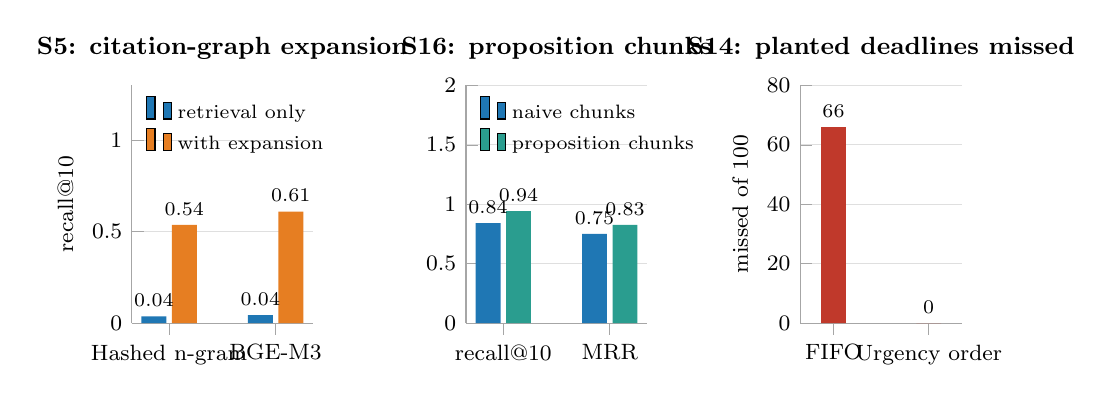
\begin{tikzpicture}
\begin{axis}[vsplot, width=0.32\textwidth, title={S5: citation-graph expansion}, ylabel={recall@10}, ymax=1.3, symbolic x coords={Hashed n-gram,BGE-M3}, xtick=data, point meta=explicit symbolic,
  nodes near coords align={vertical}]
\addplot[fill=cA, draw=none] coordinates {(Hashed n-gram,0.037) [0.04] (BGE-M3,0.043) [0.04]};
\addplot[fill=cB, draw=none] coordinates {(Hashed n-gram,0.537) [0.54] (BGE-M3,0.610) [0.61]};
\legend{retrieval only, with expansion}
\end{axis}
\begin{axis}[vsplot, at={(0.35\textwidth,0)}, width=0.32\textwidth, title={S16: proposition chunks}, ymax=2.0, symbolic x coords={recall@10,MRR}, xtick=data, point meta=explicit symbolic]
\addplot[fill=cA, draw=none] coordinates {(recall@10,0.842) [0.84] (MRR,0.751) [0.75]};
\addplot[fill=cC, draw=none] coordinates {(recall@10,0.942) [0.94] (MRR,0.826) [0.83]};
\legend{naive chunks, proposition chunks}
\end{axis}
\begin{axis}[vsplot, at={(0.70\textwidth,0)}, width=0.30\textwidth, title={S14: planted deadlines missed}, ylabel={missed of 100}, ymax=80, symbolic x coords={FIFO,Urgency order}, xtick=data, point meta=explicit symbolic]
\addplot[fill=cE, draw=none] coordinates {(FIFO,66) [66] (Urgency order,0) [0]};
\end{axis}
\end{tikzpicture}
\caption{Offline studies, no language model. Left: expanding the citation graph raises recall@10 on a self-supervised proxy (150 queries; 75 queries gained and none lost on hashed vectors). Middle: proposition-sized chunks against naive chunks on the dropout target (292 orders). Right: a simulation of 100 batches with a planted deadline; urgency order misses none.}
\label{fig:studies}
\end{figure*}


\paragraph{Label-source sensitivity.} The same outputs are scored against the agreed gold, one labeler alone and the keyword rules alone (Table~\ref{tab:table_label_sensitivity}). The ordering of the systems does not change: Full's factor recall stays below B0, B1 and B4 under the keyword rules (0.28 against 0.50, 0.61 and 0.67), under one labeler alone (0.33 against 0.44, 0.56 and 0.67) and under the agreed labels (0.25 against 0.50, 0.63 and 0.63), on 8 to 9 orders each, and every interval overlaps. The conclusion that factor recall is unresolved at this size does not depend on the label source.


\paragraph{Cost.} \resref{table9_cost} gives tokens, store calls, latency and USD per case. Full costs \$0.0107 a case (101,860 tokens, 104 store calls, 280 seconds) against \$0.0138 for B4 (131,239 tokens, a token ratio of 0.78, below the 1.0 to 1.6 the plan expected) and \$0.0004 for B0 (3,862 tokens, about 26 times fewer).


\section{Challenges and Mitigations}
\label{sec:challenges}

Table~\ref{tab:challenges} lists what went wrong while building and running the system, how each problem was found, what we did about it, and what is left to do. The hardest were running out of free-tier quota and disk, a privacy boundary that refuses some orders for hosted models, and gold labels that cover only a few development orders.

\begin{table*}[!t]
\centering\small
\begin{adjustbox}{max width=\textwidth}
\begin{tabular}{@{}p{4.6cm}p{5.4cm}p{5.2cm}@{}}
\toprule
Challenge & What happened & Mitigation \\
\midrule
Budget for hosted models & The plan needs about 4,500 Full case-runs; a Full case takes about 50 model calls. 4.15\,USD (OpenAI) and INR 5.49 (Sarvam) were spent, then both providers were locked in code. & Hosted runs moved to the Gemini free tier (500 requests a day per project per model), with a quota ledger and resumable shards; sample sizes are cut, never features; team keys are pooled. \\
Free-tier reliability & Gemma 4 31B failed on 86 of 94 calls in an hour (HTTP 500, 503); \texttt{gemini-3.5-flash-lite} rejected the default thinking setting with a bare 400. & Model chosen on a 3-case smoke (no failures on \texttt{gemini-3.5-flash-lite}); per-model thinking settings live in configuration; a case that hits the daily quota is not saved and reruns. \\
GPU serving & Qwen3-32B installed on the shared GPU nodes but never answered a prompt: the account limit on job starts blocked it. & Dropped for now; BGE-M3 vectors were built on the nodes (2\,h\,43\,min) and applied locally. \\
Thin input facts & The facts part of many orders is short or only a caption (19 of 50 dev orders under 1,000 characters). & Answerable-factor rule; coverage columns; cases with no facts are reported, not dropped. \\
Privacy refusals on hosted calls & The boundary refused some dev orders for hosted models (8 of the first 25; 26 of 100 baseline case-runs), and the local fallback model was not running, so those cases saved an error and were scored as empty briefs. & The scorer counts errored cases explicitly; every paired comparison uses only the cases both arms answered; running a local fallback model is a phase-2 fix. \\
Sparse scorable gold & Only 8 of 50 dev orders have a gold factor that the facts make answerable, 20 have an agreed objection, and none has a resolved court citation. & Every cell reports its number of cases; a 24-order set chosen from gold labels alone was used for the current-code runs; recall of cited precedents is measured in the offline studies and on the test slice only. \\
Scoring time & MiniCheck runs on a laptop CPU: scoring one block of about 500 case-runs took over three hours. & Scoring runs unattended, one model family at a time; the larger blocks are scored for the final report. \\
Gold independence & The model labeler is the same model as the system in the OpenAI runs. & Rule-only gold reported beside the agreed gold; the phase-5 runs use a different model family from the labeler. \\
Checker circularity & The unsupported-fact metric first fell back to the system's own DeBERTa checker. & The scorer now uses MiniCheck and refuses the system's checker. \\
Privacy on the wire & Names were scrubbed but FIR numbers, police stations and dates went out. & Quasi-identifier aliasing and a per-case date shift; per-case consent for client text; free tiers take public text only. \\
Rights rules not verified & Six of seven rules await a check against the bare acts; one rule's store text is wrong. & Verification bound to a hash of rule text and code; exports print ``Not yet checked against the bare act''. \\
Gated data & HLDC (Hindi district-court bail orders) and an Indic translation model are gated. & Native Hindi High Court orders as T2's Hindi set; access requested. \\
Disk & The laptop is at 97\% disk use. & Caches cleared; large weights not in use are candidates for removal. \\
\bottomrule
\end{tabular}
\end{adjustbox}
\caption{Challenges met so far and how each is handled.}
\label{tab:challenges}
\end{table*}

\section{Limitations and Risks}

\begin{itemize}\setlength\itemsep{0pt}
\item \textbf{Small $n$, dev only, one backend, superseded code.} The scored runs use the 50 dev orders on one hosted model and come from the tag \texttt{dev-sweep-v1}; later code (privacy, providers, the fixes of Section~\ref{sec:status}) has not been rerun. Intervals are wide (about $\pm$7 points at $n=50$, above the 5-point margin), and the blind slice is unopened, so no claim can be called supported.
\item \textbf{Stand-in models.} Offline arms use a template LLM; such numbers carry that label in the tables. The 4B and 14B models of the design have not been run on the GPU nodes for this report; serving Qwen3-32B on the shared nodes failed and was dropped.
\item \textbf{Thin facts in T1.} The facts part is often only a caption. A single pass then answers ``no facts supplied'', while Full draws grounds from retrieved authorities not tied to the client's facts, so Full can win on recall through retrieved boilerplate.
\item \textbf{Gold is not human.} Rules plus one non-Qwen labeler that must agree; $\kappa$ is 0.60 for G1, and the agreed G1 gold leaves 81 of 250 orders without a factor. Only 37.3\% of citations resolve, and no dev order has a resolved court citation. HLDC was unavailable, so the Hindi set is native High Court orders from one court and two years.
\item \textbf{Rights Radar.} Six of the seven rules are unverified. A rule's verification is now bound to a hash of its text and code, so a later change clears it, and every unverified rule is printed in the export as ``Not yet checked against the bare act''. T4 is generated from the same rule table, so it measures conformance, not legal accuracy.
\item \textbf{No authentication.} The gates are enforced in code, but there are no user accounts and the API token is off by default, so ``approval only from counsel'' is a property of the code path, not of an identity check.
\item \textbf{Budgets.} Spent so far: 4.15 USD on OpenAI and INR 5.49 on Sarvam; both are now locked in code. The free Gemini tier allows 500 requests a day per project on the flash-lite models, about 10 Full cases a day (a Full case takes about 49 requests). The full plan (about 4,500 Full case-runs) does not fit, so sample sizes are cut, not features.
\item \textbf{Known weaknesses.} Grounds are sometimes weak in substance (about ten open issues per case; sparring objections mostly unanswered); the pseudonymiser still refuses one order of 250.
\end{itemize}

\section{Threats to Validity}
\label{sec:threats}

\paragraph{Internal.} Small $n$ and a single run for most arms limit what can be resolved; an effect smaller than the interval is reported as not resolved. Thresholds fixed on 50 orders may be mis-set, so margins are rounded to whole points; the pass bar and NLI threshold are provisional until the freeze.

\paragraph{Construct.} Gold from rules plus an LLM labeler, not humans, risks circularity. The labeler is the same model as the system in the dev runs, so its reading of a factor and the drafter's may share biases; the rule-only gold is reported beside the agreed gold for this reason. A second circularity: the system reads the facts part of an order while gold is read from other parts of the same order, and the tagger that builds paragraph metadata is of the same family as the rule labeler. Controls are an 8-word-overlap check, agreed labels, label-source sensitivity, and B6 not reusing the tagger. Because T1 facts are often only a caption, retrieved boilerplate can inflate recall; the answerable-factor rule and the faithful/corroborated table are guards, not a cure. Factor recall against G1 measures what the defence argued, not what a good lawyer should argue; lenient precision against G1 $\cup$ G5 corrects this in part. The unsupported-fact checker (MiniCheck) is independent of the system's checker but was validated on other domains, so subtle legal entailment errors may pass.

\paragraph{External.} One legal domain (bail), one source of orders, one court for the Hindi native set, and constructed data for T2 to T5, T7 and T8 limit transfer. Only 5.9\% of orders split cleanly, so results hold for orders that split cleanly. Qwen3 and the hosted labeler may have seen public orders; the release date bounds the cutoff but does not measure it. There is no user study, and no claim about lawyer time or outcomes.

\section{Status and Plan}
\label{sec:status}

\paragraph{Done.} The six agents and the event log; the ten stores; the ingestion ladder; contracts and Sutradhar; Vakeel's check and repair; Abhiyojak; truth maintenance with the byte-identity test; Pairokar; the Rights Radar (rules unverified); both gates and the privacy boundary; the web interface and API routes. For evaluation: test sets T1 to T9, gold G1 to G7 (Table~\ref{tab:kappa}), baselines B0 to B6, every S/A/P variant as a switch (61 of 61 pass an offline end-to-end audit; 42 effect tests), the scoring pipeline (bootstrap, Wilcoxon, McNemar, cluster bootstrap, Holm), the label-source sweep, the offline studies, the code stamp in every manifest, and spend ledgers for both hosted providers. On 29 October the test suite (run per area; the fine-tuning folder excluded) gave 5,082 passed and 0 failed: 4,665 unit, 133 integration and 284 system tests; 5,264 tests are collected after the changes of that day. Since the first draft of this report the team locked the paid providers in code and moved hosted calls to the Gemini free tier (providers are added by configuration), added per-case consent and quasi-identifier aliasing to the privacy boundary, bound Gate 2 to a hash of the approved brief, bound each Rights rule's verification to a hash of its text and code, made the unsupported-fact metric use MiniCheck and refuse the system's own checker, and built BGE-M3 side vectors for the four vector stores.

\begin{table}[!t]
\centering\small
\begin{adjustbox}{max width=\textwidth}
\begin{tabular}{@{}p{3.6cm}p{1.5cm}p{1.5cm}@{}}
\toprule
Item & State & Owner \\
\midrule
Dev baselines B0--B4, B6 on the earlier code (50 cases) & done, scored & Vishak \\
Full, B0--B4, A1--A3, A6--A9 on current code (OpenAI) & run; scoring in progress & Vishak \\
B5, S1--S6, S8--S12, S15, S18 (OpenAI, 10 cases) & run; scoring in progress & Vishak \\
Gemini family: Full, B0--B3, B0L, A1, A2, A8 & run; scoring in progress & Vishak \\
A4, A5, A10, S7, S11b/c, S12b, S15b, S17, P5--P8 & not yet run & Vishak, Satvik \\
Offline studies S4/S5, S14, S16 & done & Vishak \\
Retrieval under BGE-M3 & measured (study only) & Vishak \\
Rights rule verification (6 of 7) & pending & Harshita \\
BNSS s.58 official text & pending & Harshita \\
Consent route and UI & not done & Shravani \\
Frontend merge & on hold & Satvik, Vishak \\
Freeze tags, pre-registration & template & all \\
Blind-slice run, once & after freeze & all \\
\bottomrule
\end{tabular}
\end{adjustbox}
\caption{Work left. Owners follow the split of the project file.}
\label{tab:status}
\end{table}

\paragraph{Where the project stands.} This is a work in progress with much already built. The six agents, ten stores, two approval gates, the Rights Radar, the pseudonymisation boundary, 46 opt-in switches for literature variants, and an evaluation pipeline with its statistics are implemented and tested (about 4,950 tests). Baselines, ablations and variants have been run on hosted models and the first scored comparisons are in Section~\ref{sec:results}; the numbers are small-sample dev results and we do not claim more from them than they show. Phase 2 (to 10 November) widens the runs, fixes the weaknesses these runs exposed, freezes the code and scores the blind slice once.

\paragraph{Code.} All code, tests, documents, the report source, run manifests and the tag \texttt{dev-sweep-v3} are in the repository \url{https://github.com/vishakkashyapk30/lma-group-project}; the work of this report is on the branch \texttt{midsub-report} (\url{https://github.com/vishakkashyapk30/lma-group-project/tree/midsub-report}). Data, model weights and keys are not in it; \texttt{make setup}, \texttt{make data} and \texttt{make models} rebuild them (Appendix, Reproducibility).

\paragraph{Timeline to 10 November 2026.} Table~\ref{tab:timeline}. Everything planned for this project, every run, table, fix and the final report, is finished by 10 November; the days after are held in reserve and are not planned. Each step depends on the one before, and the free-tier quota sets the pace, so dev and test runs use every teammate's key.

\begin{table}[!t]
\centering\small
\begin{adjustbox}{max width=\textwidth}
\begin{tabular}{@{}p{1.5cm}p{4.2cm}p{1.2cm}@{}}
\toprule
Dates & Step & Owner \\
\midrule
31 Oct--2 Nov & Finish the dev runs on Gemini and OpenAI (A4, A5, S11b, S11c, S12b, S15b, S7, P5--P8, A10 offline); score with MiniCheck; fill every table & Vishak, Satvik \\
1--3 Nov & Rights rules re-checked; BNSS s.58 text; consent route and UI; frontend merge & Harshita, Shravani, Satvik \\
3--4 Nov & Fix thresholds on dev; fill the pre-registration; tags \texttt{prereg-v1}, \texttt{eval-freeze-v1} & all \\
5--7 Nov & Test runs from the freeze tag: open slice, then the blind slice once (Full and B0--B4; size set by the pooled quota) & Vishak, Satvik \\
7--9 Nov & Scoring, Holm tables, failure taxonomy, case studies; final report written from the frozen tables & Harshita, Shravani, Vishak \\
10 Nov & Code freeze; repository and tags pushed; report submitted & all \\
\bottomrule
\end{tabular}
\end{adjustbox}
\caption{Plan from the mid-project checkpoint to the final submission.}
\label{tab:timeline}
\end{table}

\paragraph{Risks.} Budget: the plan needs more calls than the caps buy, so sample sizes shrink first and features never (cut order is in the plan). Compute: shared GPU nodes, where serving the 32B model failed, and a laptop with about 97\% disk use. Free-tier reliability: one model (Gemma 4 31B) failed on 86 of 94 calls in an hour, so model choice is driven by availability. Gated resources: HLDC and an Indic translation model are not yet available. Gold quality: low agreement on two factors may force a merge of confusable factors. A null result on any claim is reported as such.

\section*{Ethics and Privacy Statement}

Client files stay on the user's machine. Text leaves it only through the pseudonymisation boundary, and only when the external-model mode and counsel's per-case consent allow it; external services are off by default, paid providers are locked in code, and free-tier services, which may use prompts to improve their products, receive public court text only. On 250 T1 orders the party-name proxy found names in 80 orders before a fix to caption-name learning and 5 after; a second change now also aliases FIR, case and crime numbers, police stations, villages, addresses and ages and shifts dates per case, and the boundary refuses the 5 orders whose names OCR glued to other words. We do not claim zero leakage: the scrubber is rule-based, and Hindi coverage is thin. Keys live in environment variables, never in the repository, and spending is capped in code. The public corpus is court text already in the public domain; orders with the same FIR as a test order are excluded from the stores. The system makes no outcome predictions, shows no grant rates, and gives no advice to accused persons or the public; the landing page points them to free legal aid (NALSA helpline 15100). Export needs counsel's approval at Gate 2. Constructed test cases use synthetic names. No manual annotation was used.


\bibliography{references}

\clearpage
\onecolumn
\newgeometry{a4paper,left=1.8cm,right=1.8cm,top=2.2cm,bottom=2.2cm}
\appendix
\section{Reproducibility}
\label{app:repro}

\paragraph{Code and data.} The repository is the code of record; the pinned tag for the current dev runs is \texttt{dev-sweep-v3} (commit \texttt{7ad6ed4}; the tag \texttt{dev-sweep-v1}, commit \texttt{efd0ce4}, is the superseded 50-case run). Data (\texttt{interim}, stores, test sets, gold, and the raw sources: Open India Law shards, IPC2BNS-Verify, Kathbath) is not in the repository. It is a private dataset in the Hugging Face organisation \texttt{Vakeel-Sahayak}, \texttt{vakeel-sahayak-data}; access is granted by the owner. Helper models (BGE-M3, DeBERTa NLI, MiniCheck, Whisper small) are fetched by \texttt{make models}.

{\footnotesize\begin{verbatim}
make setup
make data
make models
make smoke        # case-0007, offline
make eval-smoke
python -m vakeel_sahayak.eval.runners.driver \
  plan --sweep
python -m vakeel_sahayak.eval.scoring score \
  --runs data/eval/dev_runs --slice dev \
  --gold-source both --out data/eval/dev_scores
python -m vakeel_sahayak.eval.scoring report \
  --scores data/eval/dev_scores
\end{verbatim}}

\paragraph{Manifests.} Each run writes a manifest with the system id and variant, prompt hash, config hash, model names and modes, test-set and gold hashes, shard count, and the code stamp (\texttt{git\_sha}, \texttt{git\_dirty}, \texttt{code\_tree\_hash}). The scoring loader refuses runs from different commits unless told otherwise, and a dirty stamp is not admissible for frozen runs. The hosted-model settings are \texttt{VS\_MODELS=auto}, \texttt{VS\_LLM\_BACKEND=openai}, \texttt{VS\_EXTERNAL=pseudonymised}, with keys read from an untracked \texttt{.env}; offline stand-ins are the default and need neither a GPU nor a key. Agreed-gold hashes: agreed-gold sha256 \texttt{5583690e3754dacd8f2ebd4e27987ae7cfa0c3df9eb2fd9e8bc9a879d86c05be}, shared by every run of the current code; code tag \texttt{dev-sweep-v3}, git sha \texttt{7ad6ed41ea39}, code tree hash \texttt{d85cdc64f123}; the 24-case file of scorable orders has cases hash \texttt{ec0611f23b3c7749}.

\section{Arms}
\label{app:arms}

\begin{table}[H]
\centering\small\setlength\tabcolsep{3pt}
\begin{adjustbox}{max width=\textwidth}
\begin{tabular}{@{}lp{5.2cm}p{3.5cm}l@{}}
\toprule
Id & Idea (source) & Switch & Run so far \\
\midrule
B0, B1, B4, B6, Full & baselines (Section~\ref{sec:eval}) & driver system id & run on the earlier code (50 cases) and the current code; scored \\
B0L, B2, B3, B5 & baselines & driver system id & run on the current code; B0L, B2 and B3 scored in the Gemini family, B5 scoring in progress\\ B0S & baseline & driver system id & not run \\
S1 & self-critique retrieval \citep{asai2024selfrag,yan2024crag} & \texttt{retrieval\_policy} & run (OpenAI); scoring in progress \\
S2 & adaptive depth \citep{jeong2024adaptive} & \texttt{retrieval\_policy} & run (OpenAI); scoring in progress \\
S3, S3b & sufficiency stopping \citep{joren2025sufficient} & \texttt{stopping} & run (OpenAI); scoring in progress \\
S4 & score-skew weak signal & \texttt{weak\_signal} & offline study \\
S5 & citation-graph expansion \citep{gutierrez2025hipporag2} & \texttt{graph\_expansion} & offline study \\
S6 & learned store prior \citep{zhang2026agentrouter} & \texttt{store\_prior} & run, no effect without a trained prior \\
S7 & hierarchy re-reading for Munshi & \texttt{munshi\_gap\_policy} & not run (T2 phase) \\
S8 & self-critique repair \citep{gou2024critic,huang2024selfcorrect} & \texttt{repair\_mode} & run (OpenAI); scoring in progress \\
S9, S10 & sampling critic; no isolation \citep{choi2025debate,wynn2025talk} & \texttt{critic\_mode}, \texttt{abhiyojak\_isolation} & run (OpenAI); scoring in progress \\
S11 & three-role review, debate, vote \citep{kumar2025courtevel} & \texttt{critic\_mode}, \texttt{draft\_mode} & S11 run (OpenAI); scoring in progress; S11b, S11c in progress \\
S12 & topology: sequential, single agent \citep{cemri2025mast} & \texttt{topology} & S12 run (OpenAI); scoring in progress; S12b in progress \\
S13 & searched workflow (grid on dev) & none (grid over switches) & offline smoke \\
S14, S14b--d & plan cache, scheduling, prefix signal \citep{zheng2024sglang} & \texttt{plan\_cache}, \texttt{urgency\_policy} & offline study \\
S15, S15b & output format \citep{tam2024speak} & \texttt{output\_format} & S15 run (OpenAI); scoring in progress; S15b in progress \\
S16, S16b & proposition units, late chunking \citep{chen2024densex} & \texttt{chunking} & offline study \\
S17 & injection defences \citep{beurerkellner2025patterns} & defence flags & not run (T7 phase) \\
S18 & authority stance \citep{wachsmuth2018} & \texttt{authority\_stance} & run (OpenAI); scoring in progress \\
P5--P8 & ingestion arms, image-only \citep{yu2025visrag,faysse2025colpali} & \texttt{munshi\_*} & not run (T2 phase) \\
A1--A10 & remove one part (dossier, repair, tools, filter, extractor, router, planner, sparring, a store) & \texttt{Switches} flags & A1 to A3, A6 to A9 run; A4, A5, A10 not run \\
\bottomrule
\end{tabular}
\end{adjustbox}
\caption{Arms and their state. ``Run'' means the arm has produced outputs on the tag \texttt{dev-sweep-v3} on the stated backend and cases; ``not run'' means it is implemented and offline-smoked but has produced no outputs. Switch names follow \texttt{orchestration/switches.py}; S18 is \texttt{authority\_stance=outcome} and S3b is \texttt{stopping=llm}.}
\end{table}

\section{Metrics}
\label{app:metrics}

\begin{table}[H]
\centering\small
\begin{adjustbox}{max width=\textwidth}
\begin{tabular}{@{}llp{6.2cm}l@{}}
\toprule
Id & Metric & Definition and check & Set \\
\midrule
M1--M3 & factor recall, precision, F1 & set comparison with G1 (and G5 for lenient precision) on answerable factors; argue-all F1 as floor & T1 \\
M4 & G5, G4, G6 recall & as M1 for court-discussed factors, objections, conditions & T1 \\
M5 & label-source sensitivity & M1 to M4 on rules-only, labeler, agreed; $\kappa$ per factor & T1 \\
M6 & unsupported-fact rate & share of factual sentences MiniCheck or the NLI finds unsupported & T1 \\
M7 & factual error & wrong section, date, statute text, custody count against tools & T1 \\
M9 & fabricated citation & id not in index, or span not found verbatim & T1 \\
M10, M11 & recall@$k$, MRR, nDCG@10 & court-cited precedents, with coverage columns & T1 \\
M12 & slot-fill rate & required slots filled; missing slots are open issues & T1 \\
M13, M15 & authority quality, good-law violations & metadata and graph lookup; known-treatment share & T1 \\
M16, M17 & citation precision, recall; removal & ALCE-style; claims unchanged when the paragraph is removed & T1 \\
M18 & stopping quality & over-search and stopped-too-early & T1 \\
M19 & weak-evidence AUROC & score skew predicts a top-10 gold hit & T1 \\
M33 & coverage-risk & abstention curve & T1 \\
Ingestion & CER, boundary F1, type and field accuracy & against construction truth; escalation, GPU seconds & T2 \\
Rights & accuracy, false-ELIGIBLE & designed answers by construction; Wilson interval & T4 \\
Safety & attack success, unapproved exports & bounded by the rule of three & T7 \\
Cost & tokens, calls, latency, USD & from manifests and ledgers; cost-quality frontier & all \\
\bottomrule
\end{tabular}
\end{adjustbox}
\caption{Metrics. Definitions are in the evaluation plan; none is an LLM-judge score.}
\end{table}

\section{Glossary of Names Used in This Report}
\label{sec:glossary}

\begin{description}\itemsep0pt
\item[Full] The complete system: all six agents, the ten stores, retrieval, verification and prosecution sparring.
\item[B0 to B6] Baselines, simpler systems that Full must beat. B0: one model call with no retrieval. B1: retrieval from one store. B2: retrieval over whole-order embeddings. B3: retrieval over naively chunked text. B4: every store searched and fused, with no agent planning. B5: a learned router alone, with no contracts. B6: rules only, no model. B0L: B0 on a larger model.
\item[A1 to A10] Ablations: Full with one part switched off, to show whether the part earns its place.
\item[S1 to S18] Variants taken from the literature (Section~\ref{sec:literature}). Each swaps one idea from a paper into the system as an opt-in switch. P5 to P8 are the same for intake.
\item[Dev set] The 50 development orders (T1 dev). All numbers in this report come from it. The blind slice has not been opened.
\item[Code tag] A named snapshot of the code. \texttt{dev-sweep-v1} (27 October) is the code of the first 50-case baseline runs; it is superseded and reported only as such. \texttt{dev-sweep-v3} (29 October) is the current code; every other model run reported here comes from it. A result is comparable only with results from the same tag, and the scorer refuses to mix tags.
\item[Block] A batch of runs on one model and one set of cases: the OpenAI block (\texttt{gpt-6-luna}), Gemini block A (\texttt{gemini-3.5-flash-lite}) and Gemini block B (\texttt{gemini-3.1-flash-lite}). Arms are compared only with the Full of the same block (Table~\ref{tab:models}).
\item[Agents] Munshi (intake), Peshkar (dossier and Rights Radar), Sutradhar (orchestrator), Vakeel (drafter), Abhiyojak (prosecution sparring), Pairokar (batch desk).
\item[Gates] Gate 1 (dossier) and Gate 2 (brief): approvals that only counsel can give; export is impossible before Gate 2.
\item[Metrics] M1 to M35, listed in the metrics table of this appendix: M1 factor recall, M6 unsupported-fact rate, M10 recall of cited precedents, and so on.
\end{description}

\section{Models and Where They Ran}
\label{app:models}

\begin{table}[H]
\centering\small
\begin{adjustbox}{max width=\textwidth}
\begin{tabular}{@{}p{4.0cm}p{2.6cm}p{4.2cm}p{1.6cm}p{5.2cm}@{}}
\toprule
Block of runs & Provider & Model & Runs & Arms and size \\
\midrule
Dev runs, code \texttt{dev-sweep-v1} (superseded) & OpenAI & \texttt{gpt-6-luna} & hosted & Full (2 runs), B0, B1, B4: 50 cases, scored; B6 is a rule baseline with no model \\
Block A (OpenAI), current code & OpenAI & \texttt{gpt-6-luna} & hosted & Full, B0 to B5, A1 to A3, A6 to A9, S1 to S6, S8 to S12, S15, S18: run, scoring in progress, not reported in this version \\
Block A (Gemini) & Google, free tier & \texttt{gemini-3.5-flash-lite}; B0L on \texttt{gemini-3.6-flash} & hosted & Full, B0 to B3, B0L: 10 cases; A1: 5; scored \\
Block B & Google, free tier & \texttt{gemini-3.1-flash-lite} & hosted & Full, A2, A8: 5 cases; run, not yet scored \\
Offline studies & none (no language model) & real stores, hashed n-gram and BGE-M3 & local & S4 and S5 (150 queries), S14 (100 simulated batches), S16 (292 orders) \\
Gold labeler & OpenAI & \texttt{gpt-6-luna} & hosted & labels the dev and test orders (public court text only); a label counts only if the rule labeler agrees \\
Claim checker (system) & local & DeBERTa NLI & local & inside Vakeel \\
Claim checker (scoring) & local & MiniCheck-RoBERTa-Large & local & evaluation only \\
Retrieval & local & hashed n-gram; BGE-M3 (study only) & local & BGE-M3 vectors built on GPU nodes \\
Speech & local & Whisper small & local & T8 \\
\bottomrule
\end{tabular}
\end{adjustbox}
\caption{Every block of runs, its provider and model, and whether it ran locally or on a hosted service. Only one model family serves as system in each block, so each comparison is paired within a block.}
\label{tab:models}
\end{table}

\section{Further Generated Tables}
\label{app:tables}

\gentable{table1a_v1}
\gentable{table1b_v1}
\gentable{main_v1}
\gentable{ablate_v1}
\gentable{main_gemini}
\gentable{ablate_gemini}

\resulttable{table_paired}{w}
\resulttable{table_holm}{w}
\resulttable{table9_cost}{w}
\resulttable{table_label_coverage}{n}
\resulttable{table_label_sensitivity}{w}
\resulttable{table_label_kappa}{n}
\resulttable{table_citations}{w}
\resulttable{table_abstention}{w}


\end{document}
